\documentclass{article}
\usepackage{amsmath}
\usepackage{graphicx}
\usepackage{hyperref}
\usepackage{xcolor}

\title{IT Workshop Internal Exam - Set 2}
\author{Question 1: Answer any 2 of the following 3 questions. Time: 2 hours. Full marks 30}
\date{July 2024}

\begin{document}
	\maketitle
	
	\section{Document Structure}
	LaTeX is a high-quality typesetting system that includes features designed for the production of technical and scientific documentation. It is widely used in academia for the communication and publication of scientific documents in many fields, including mathematics, computer science, engineering, physics, chemistry, economics, and political science.
	
	\subsection{Font Styles}
	Here are some examples of different font styles in \LaTeX:
	\begin{itemize}
		\item \textbf{Bold text}
		\item \textit{Italic text}
		\item \underline{Underlined text}
		\item \~{} - Tilde
		\item \^{} - Caret
		\item \textbackslash{} - Backslash
	\end{itemize}
	
	\subsection{Special Characters}
	LaTeX allows you to include special characters such as:
	\begin{itemize}
		\item \# - Hash
		\item \$ - Dollar sign
		\item \% - Percent sign
		\item \& - Ampersand
		\item \_ - Underscore
		\item \{ - Left curly brace
		\item \} - Right curly brace
	\end{itemize}
	\subsection{Including Figures}
	To include figures, you first need to upload the image file named sample-image from your computer using the upload link in the file-tree menu. Then use the include graphics command to include
	it in your document	
	
	
	\subsection{Creating Tables}
	Here is an example of creating a table in \LaTeX:
	\begin{table}[h]
		\centering
		\begin{tabular}{|c|c|c|c|}
			\hline
			Country & Primary Education & Secondary Education  &  Higher Education\\
			\hline
			USA & Grades 1-5 & Grades 6-12 & College/University \\
			\hline
			UK & Years 1-6 & Years 7-13 & College/University\\
			\hline
			India & Grades 1-5 & Grades 6-12& College/University \\
			\hline
		\end{tabular}
		\caption{Comparison of Basic Education Systems}
	\end{table}
		
	
	\subsection{Mathematical Expressions}
	LaTeX excels at typesetting mathematics. Here is the quadratic formula inline: \( ax^2 + bx + c = 0 \).
	
	Displayed version: 
	\[
	\begin{pmatrix}
		a & b \\
		c & d \\
	\end{pmatrix}
	\begin{pmatrix}
		e & f \\
		g & h \\
	\end{pmatrix}
	=
	\begin{pmatrix}
		ae + bg & af + bh \\
		ce + dg & cf + dh \\
	\end{pmatrix}
	\]
	
	Definite Integral:
	\[
	\int_0^1 x^2 \, dx = \left[ \frac{x^3}{3} \right]_0^1 = \frac{1}{3}
	\]\\
	\begin{figure}
		
		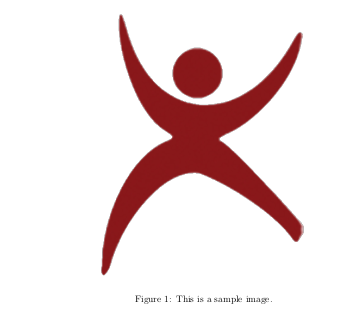
\includegraphics{r.jpeg}
	\end{figure}
	\subsection{Lists}
	You can make lists with automatic bullet points:
	\begin{itemize}
		\item First item (apple)
		\item Second item (banana)
		\item Third item (cherry)
	\end{itemize}
	
	You can also use numbered lists with colored text:
	\begin{enumerate}
		\item \textcolor{blue}{Blue}
		\item \textcolor{blue}{More blue}
		\item \textcolor{red}{And red!}
		\item \textcolor{green}{This is green color}
	\end{enumerate}
	
	\subsection{Hyperlinks}
	For more information, visit the \href{https://www.latex-project.org}{LaTeX project website}.
	
	\subsection{Bibliography}
	To include references, you can use BibTeX. Here is an example citation: \cite{Doe24}.
	
	\begin{thebibliography}{9}
		\bibitem{Doe24}
		John Doe,
		\textit{An example article},
		Journal of Examples,
		1(1):1--2,
		2024.
	\end{thebibliography}
	
\end{document}